\documentclass{article}
\usepackage{enumitem}
\usepackage{graphicx}
\usepackage{grffile}
\usepackage{float}
\begin{document}
\title{%
 Deliverable 5\\
 \large An explanation of the system, information on implementation and\\
 \large conclusion of the project
}
\author{Epic Group}
\date{}
\maketitle

\section*{Introduction}
The purpose of this report is to provide a summary and update on the status of
CinemaScout, the ultrafast movie search tool. The report will contain the following
components:
\subsubsection*{Part 1}
\begin{enumerate}
\item \textbf{System Summary}: An explanation of the purpose of the system
and the problems addressed, including problem statements.
\item \textbf{Feature List}: An enumeration over a list of features currently
implemented.
\item \textbf{User Stories}: An updated list of user stories relating to the
previous report.
\item \textbf{Final Interface}: A series of screenshots capturing the final
implementation of the interface.
\end{enumerate}
\subsubsection*{Part 2}
\begin{enumerate}
\item \textbf{Implementation Summary}: A summary on the requirements of
implementation and its current deployment status.
\item \textbf{Software Architecture}: A description of the software
architecture currently implemented via ER and UML diagrams.
\item \textbf{Sequence Diagrams}: A series of sequence diagrams for
use cases of CinemaScout.
\item \textbf{Design Outcomes}: A summary of the benefits the current 
implementation of CinemaScout provides.
\end{enumerate}
\subsection*{Part 3}
\begin{enumerate}
\item \textbf{Team Organisation}: A description of the responsibilities and
organisation of the team.
\item \textbf{Issues}: A series of technical and non-technical problems
encountered.
\item \textbf{Project Reflection}: A final reflection over the outcome of the
course.
\end{enumerate}

\section{Part 1}
\subsection{System Summary}
CinemaScout is a movie search tool which aims to provide a faster and more
accurate method of receiving movie suggestions. This is achieved 
through the rectification of a number of harmful design choices made by other 
movie suggestion platforms, most often in place as an unintended consequence 
of centralisation. These include the following problem statements:
\begin{itemize}
\item \textbf{Restricted Movie Database}: Only movies which are available for
viewing on the same platform are recommended, restricting the scope of movies
available.
\item \textbf{History Poisoning}: Movie recommendations are based on previous
browsing history or via similar metadata, producing unwanted and erroneous
movie suggestions due to the indeterminant browsing habits of most users.
\item \textbf{Low Computational Requirement}: Movie recommendation is often a
smaller, neglected module of a larger platform, elliciting a low computational 
requirement and therefore poor quality results.
\item \textbf{User Registration Requirement}: Movie recommendation platforms
often gratuitously require users to register before the use of a service is
allowed, needlessly creating the opportunity for user data to be leaked through
inevitable database leaks and security breaches.
\item \textbf{User Sanitisation Requirement}: Movie recommendation platform
algorithms rely on user input to function, enabling the insertion of dangerous
or illicit content to other users by malicious actors.
\item \textbf{Corporate Bias}: Private business deals between platforms force
suggestions to benefit its business partners, degrading the quality and
integrity of results.
\end{itemize}
\subsection{Feature List}
Principally, CinemaScout provides the ability for a user to traverse the entire
IMDb database via a procedurally generated questionaire. The questionaire 
enables a user to identify an extremely specific and unique subset of high
quality movies. In addition, CinemaScout provides the following auxillary 
features:
\begin{itemize}
\item \textbf{Automatic Exclusion}: The ability for a search to preemptively 
remove movies based on commonly disliked criteria.
\item \textbf{Search Progress Bar}: A progress bar which represents the amount
of movies which have been filtered by the questionaire so far.
\item \textbf{Current Best Result}: A repeatedly updating hint describing a
movie which the questionaire references.
\item \textbf{Additional Information}: Additional information for each
movie such as year, runtime, plot, director and many more.
\item \textbf{Movie Posters}: The official poster image for each movie as a 
visual guide for easy identification.
\item \textbf{Results Table}: A condensed, tabulated form of the results.
Movies can be sorted by name, year, rating, popularity and runtime.
\item \textbf{Print Results}: The ability to print the results in an easy to
read format.
\item \textbf{Save Results}: The ability to save results, which remain 
persistent between browser, computer and server restarts.
\end{itemize}
\subsection{User Stories}
The following user stories have been corrected, primarily to accomodate for the
`View Saved Search' button and the lack of a feasbile way to present
trailers of movies due to YouTube API restrictions. The user stories now
correctly reflect the final stage of the design.
\begin{itemize}
\item \textbf{User Story}: As an avid film watcher, I want to receive
tailored, specific recommendations relevant to me.
\newline \textbf {Scenario:} Given that I am on the website and that I perform
a movie search, when I receive results, then I should see results which are
most relevant to me.

\item \textbf{User Story}: As someone who enjoys multiple movie genres, I want
to receive recommendations which are not based on my previous viewing sessions.
\newline \textbf {Scenario:} Given that I am on the website and I have
previously made a search and I perform a new search, when I receive results,
then the results should not be an amalgamation of my previous sessions.

\item \textbf{User Story}: As a power user, I wish to be able to receive many
movie recommendations over a short period of time.
\newline \textbf {Scenario:} Given that I have performed many searches recently,
and I want to perform a new search, when I receive results, then the new
results are not rate limited.

\item \textbf{User Story}: As a first time website visitor, I wish to be able
to perform a search without offering my credentials and other personal
information to first generate an account.
\newline \textbf {Scenario:} Given that I have visited the website, and I want
to make my first search, when I attempt to search, then I am not prompted
to first create an account.

\item \textbf{User Story}: As a user of the service, I wish to be able to use
the service in its full capability without malicious content from ever
corrupting my movie suggestions.
\newline \textbf {Scenario:}  Given that I have visited the website, and I make
my search, when I receive my results, then the results should be free from user
generated content.

\item \textbf{User Story}: As a user of the service, I do not wish to receive
recommendations based on corporate interests or monetary influence.
\newline \textbf {Scenario:} Given that I have visited the website, and I make
my search, when I receive my results, then the results should be free from
corporate bias.

\item \textbf{User Story}: As a returning user of the service, I wish to be able
to view my recommendations and come back to my search results later.
\newline \textbf {Scenario:} Given that I am on the website, and I have
previously made and saved a search, then I can return back to the result page 
and view my former results by clicking `View Saved Seach'.

\item \textbf{User Story}: As a user of CinemaScout who wants to print out my
results, I wish to be able to print out a formatted version of the results page
tailored for readability on an A4 page.
\newline \textbf {Scenario:} Given that I am on the result page, and I click
`Print Results', then a prompt to print my results will be opened.

\item \textbf{User Story}: As a user of CinemaScout who wishes to view
the results of the search offline, I want to be able to download the search
results in a readable format for offline use.
\newline \textbf {Scenario:} Given that I am on the result page, and I click
`Print Results', then a PDF copy of the current page may be copied via the
browser.
\end{itemize}
\newpage
\subsection{Final Interface}
All images were captured at a resolution of 1920 x 1080 using a default
Chromium browser on Arch Linux. This implementation of CinemaScout was captured
at cinemascout.xyz.
\begin{figure}[H]
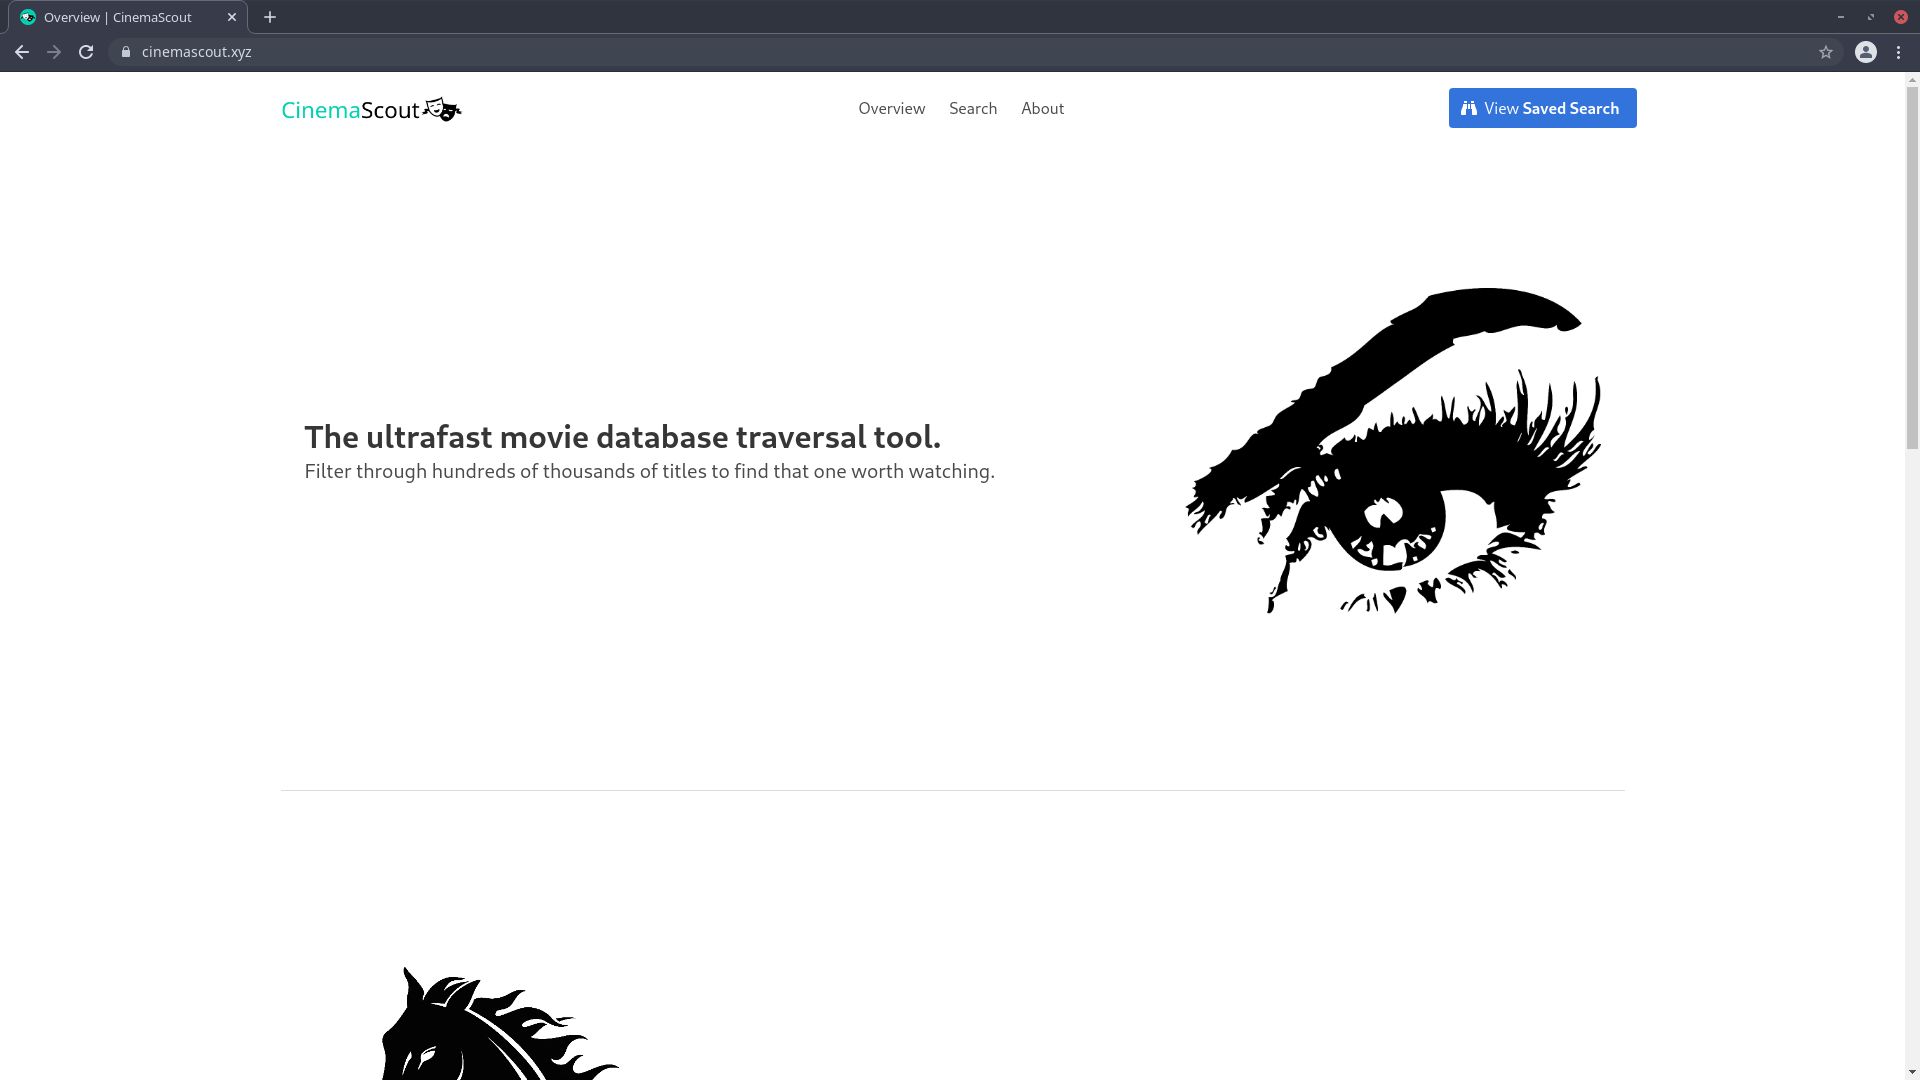
\includegraphics[width=\columnwidth]{res/main_0.png}
\caption{Landing page.}
\end{figure}
\begin{figure}[H]
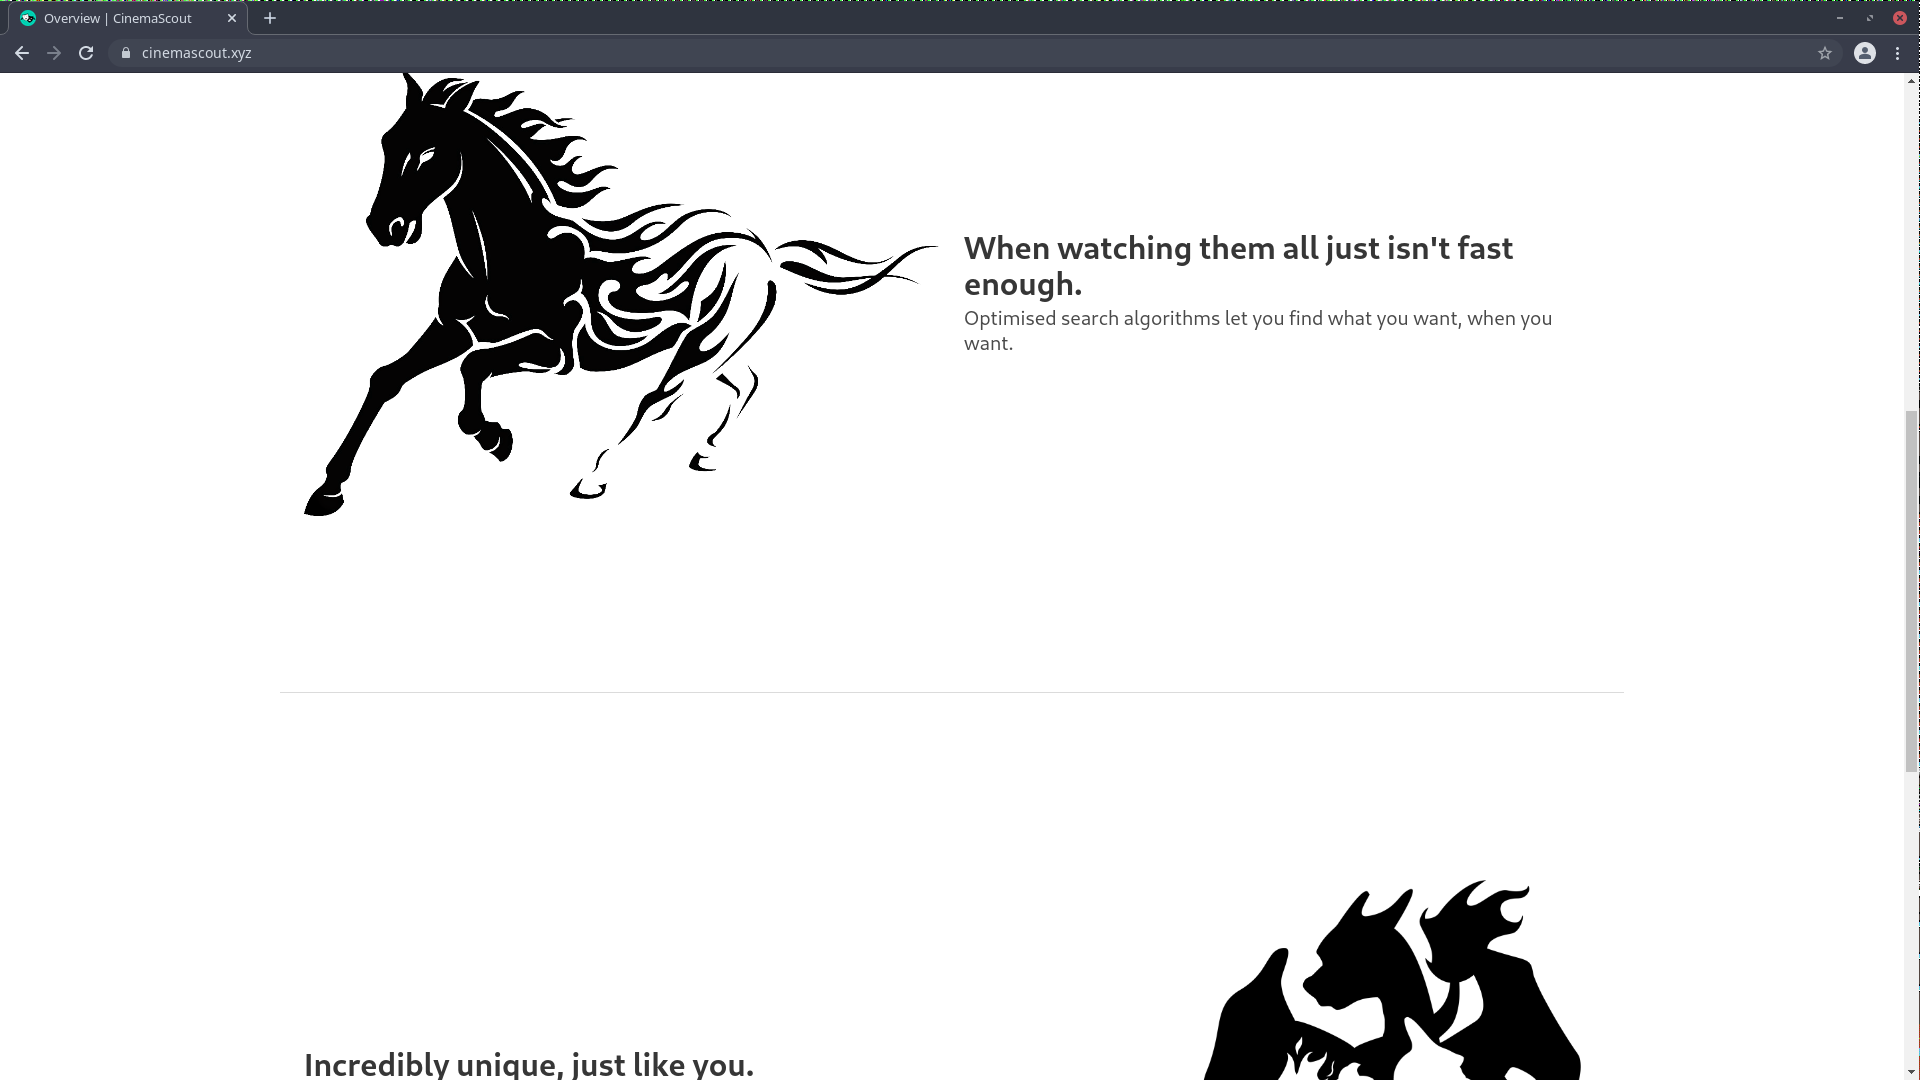
\includegraphics[width=\columnwidth]{res/main_1.png}
\caption{Middle of landing page.}
\end{figure}
\begin{figure}[H]
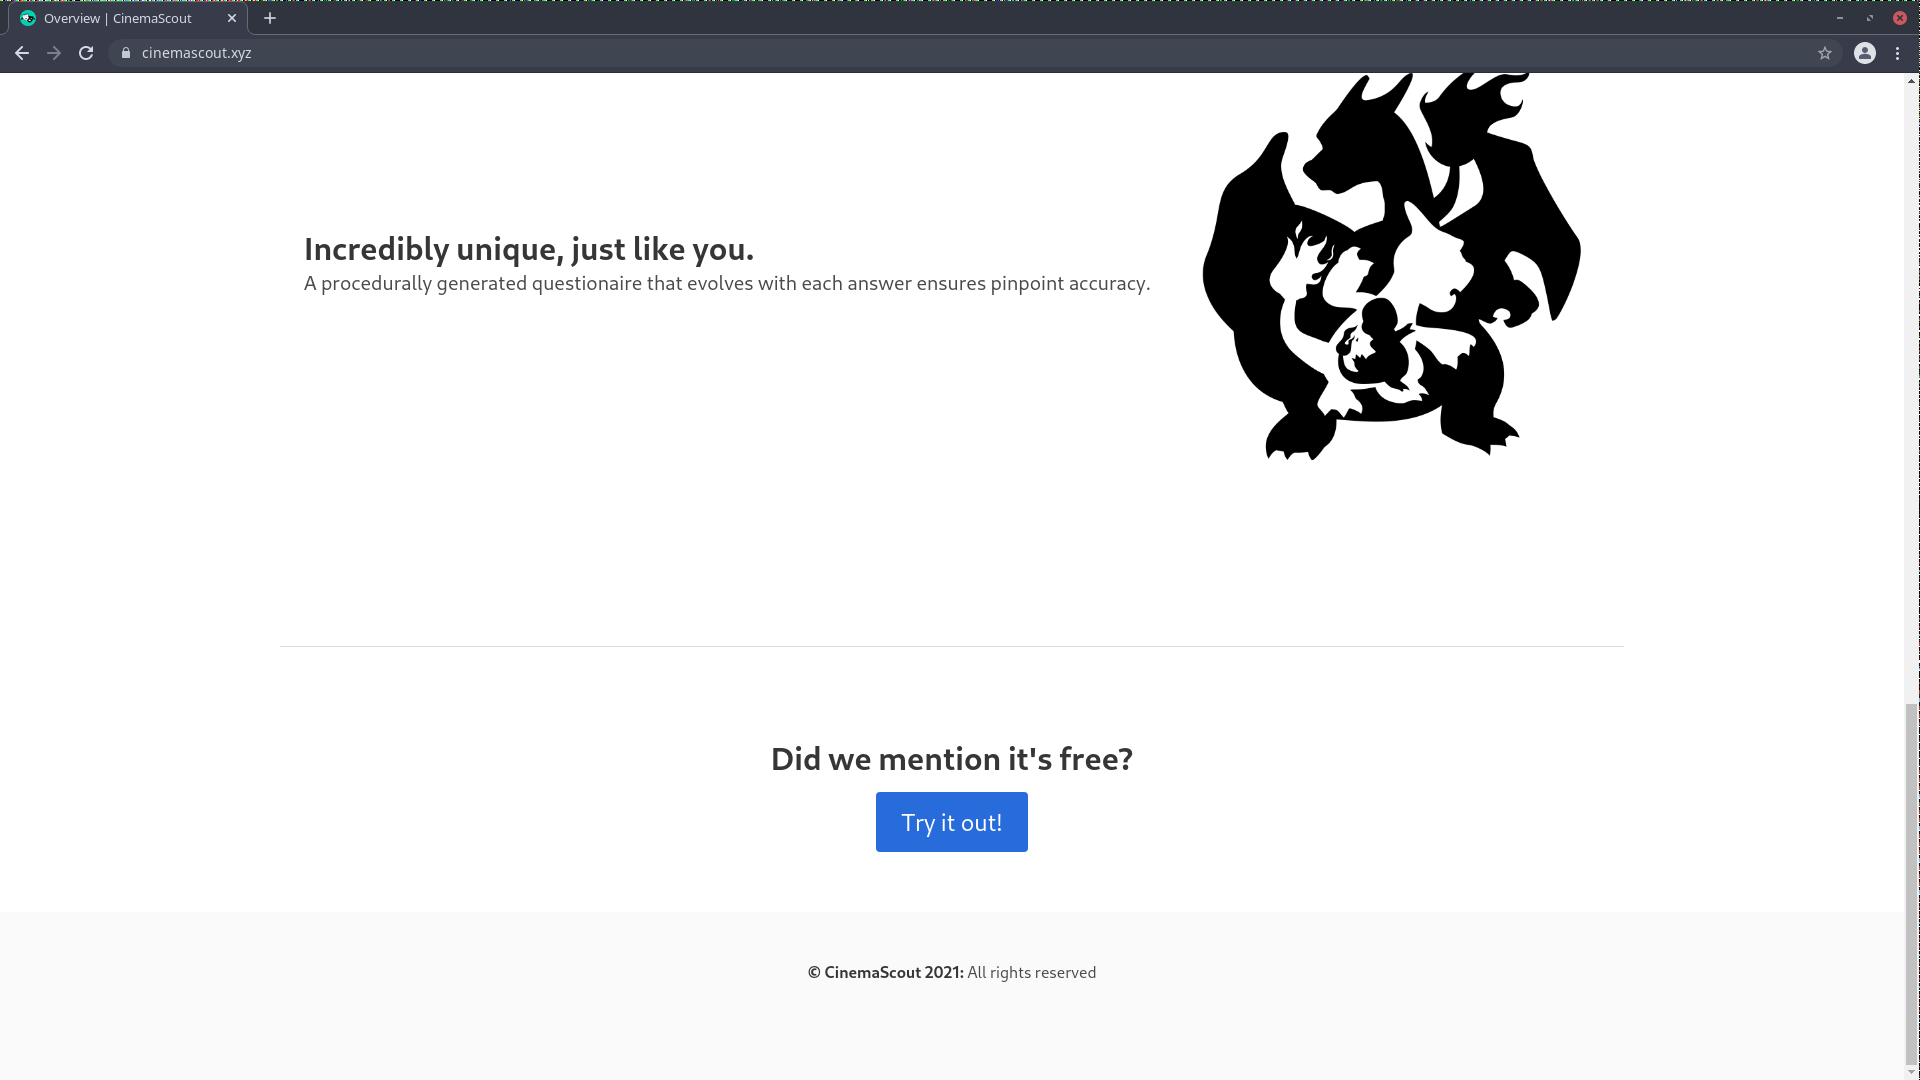
\includegraphics[width=\columnwidth]{res/main_2.png}
\caption{End of landing page.}
\end{figure}
\begin{figure}[H]
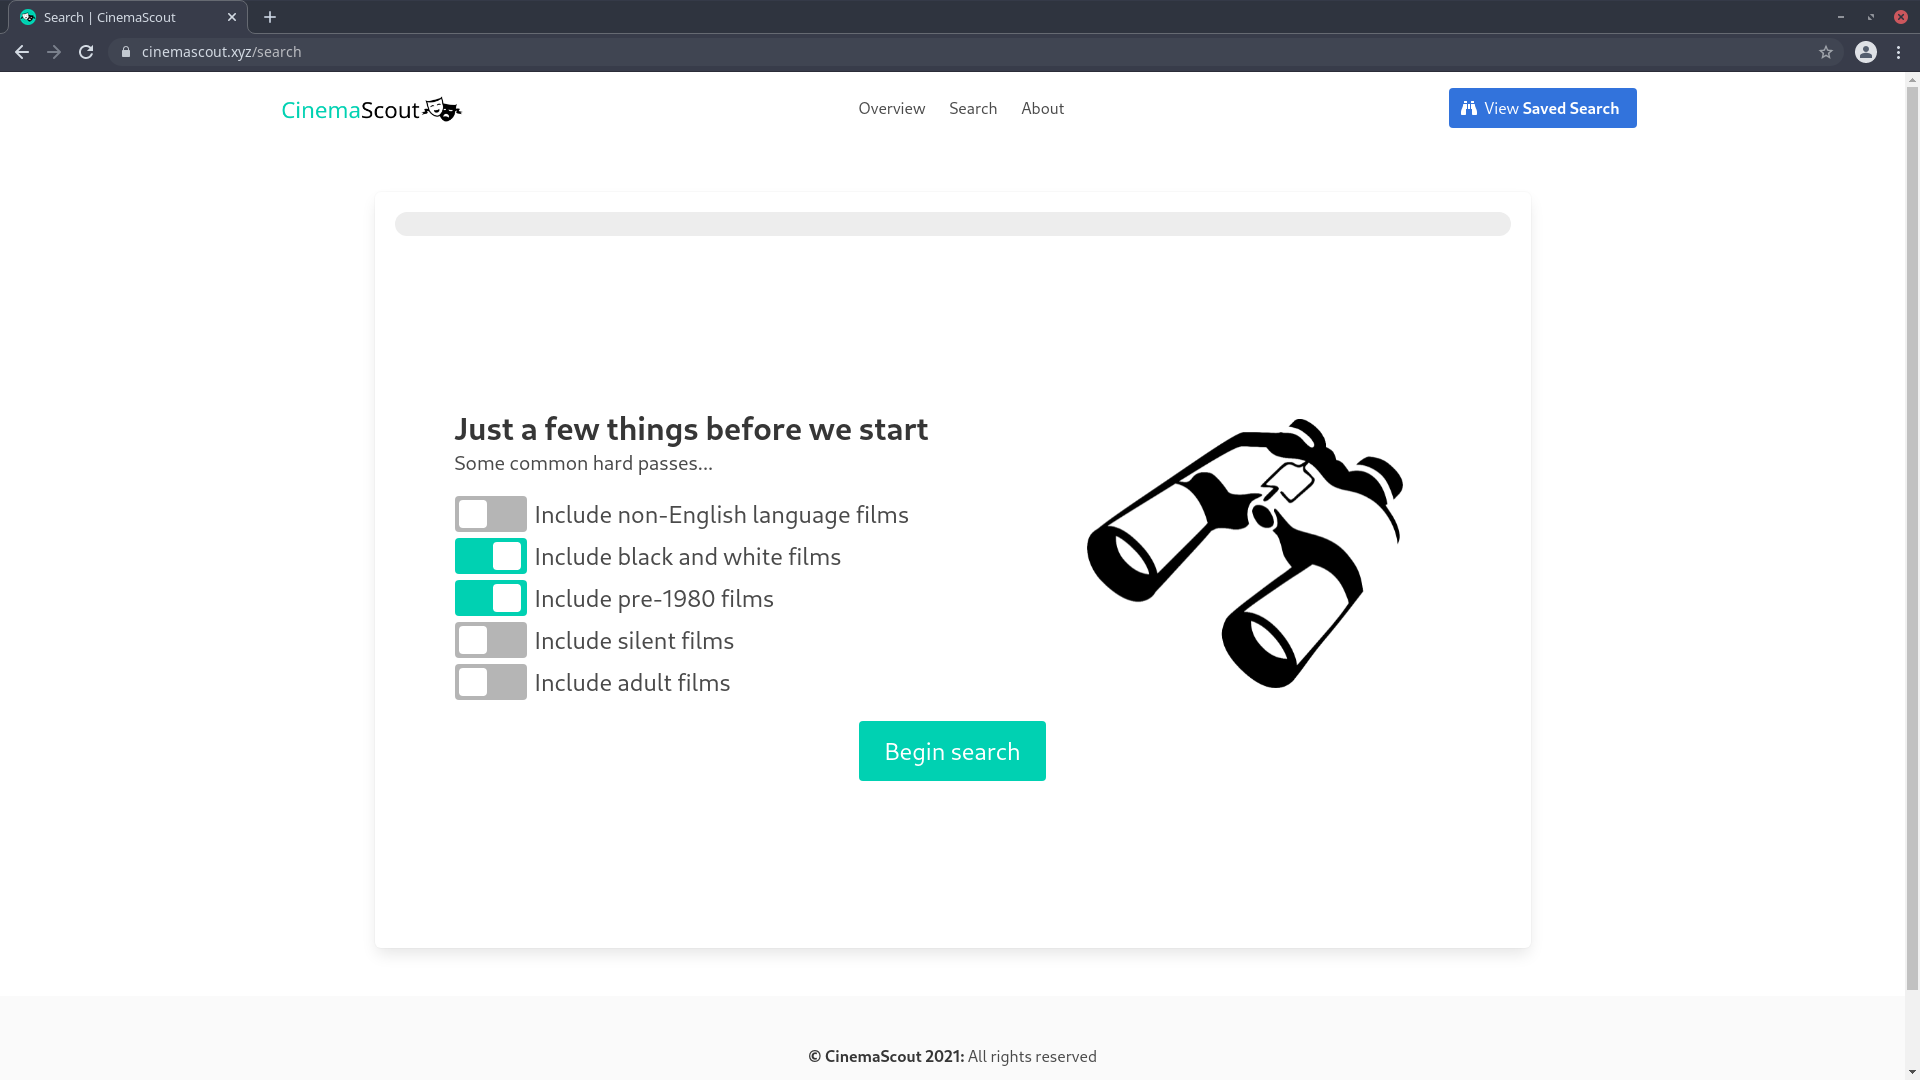
\includegraphics[width=\columnwidth]{res/search_0.png}
\caption{Search page, without further user input.}
\end{figure}
\begin{figure}[H]
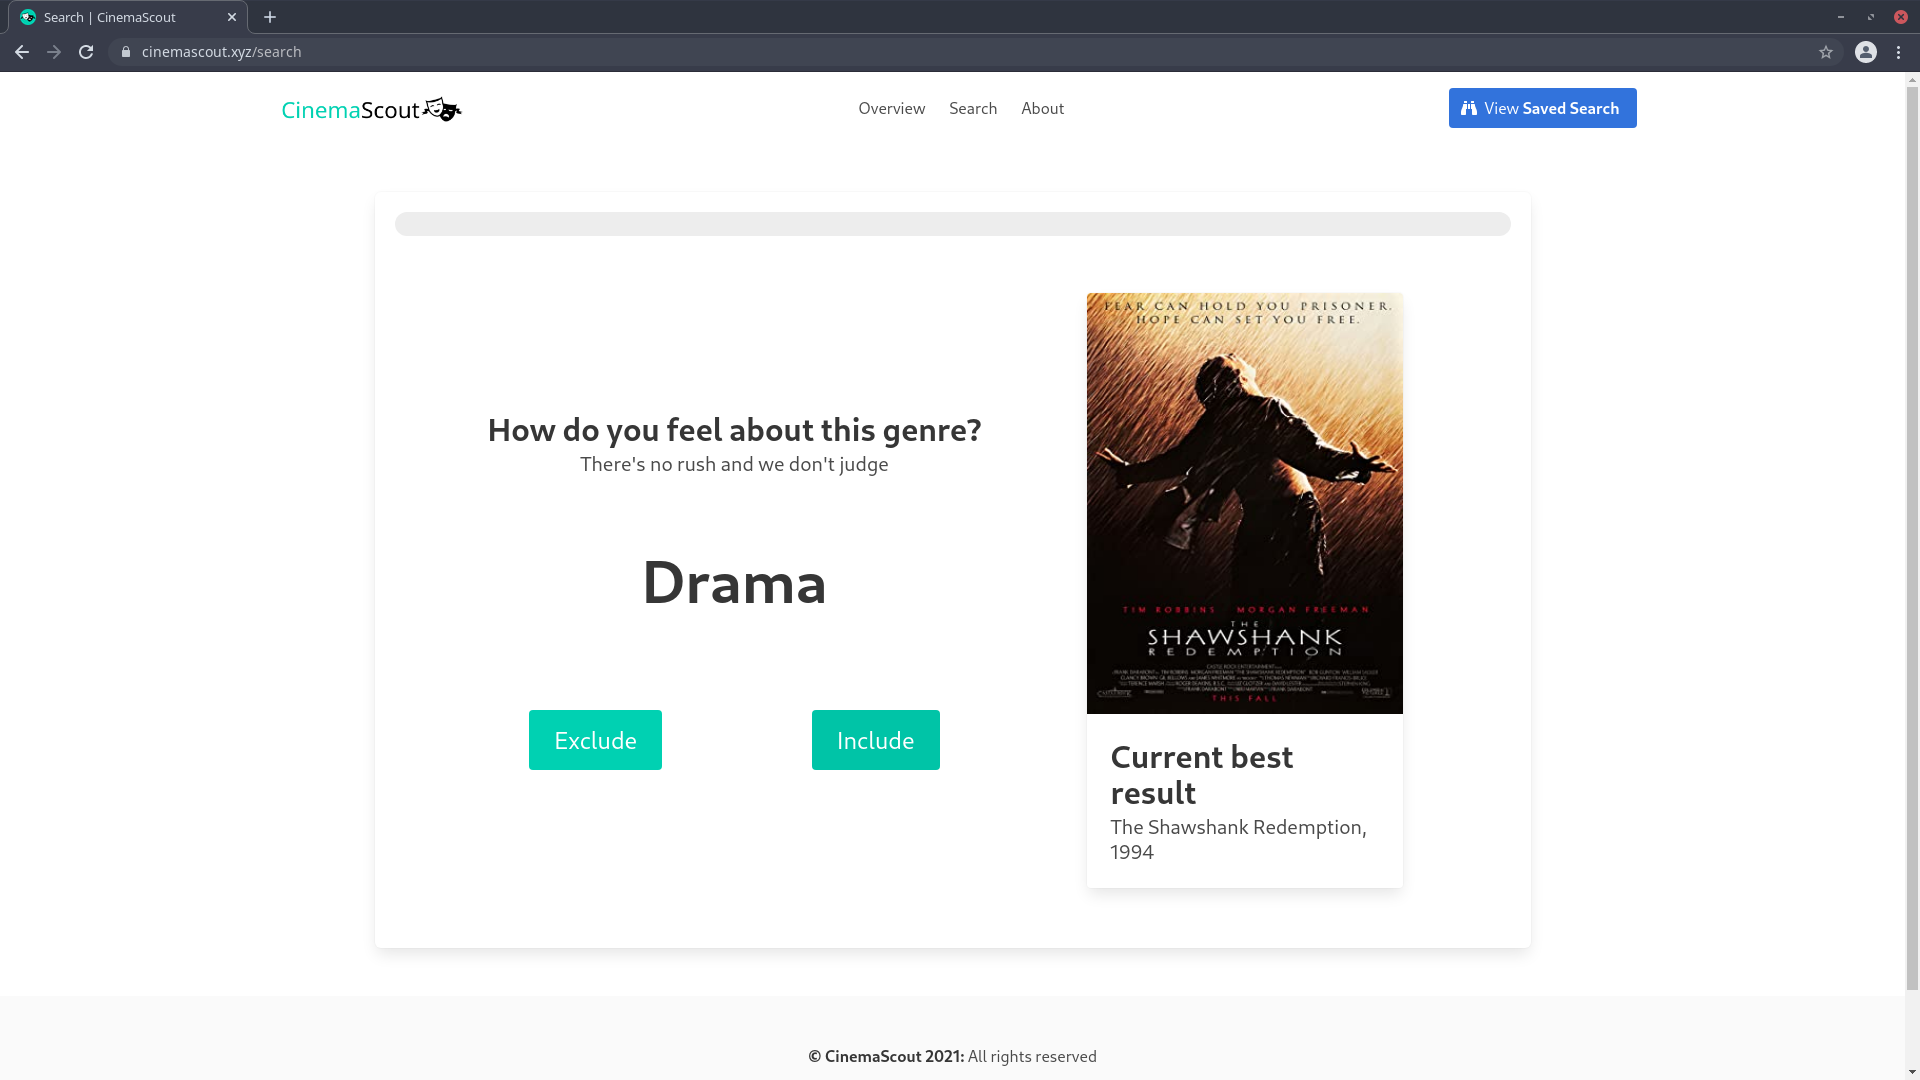
\includegraphics[width=\columnwidth]{res/search_1.png}
\caption{Search page, during a search.}
\end{figure}
\begin{figure}[H]
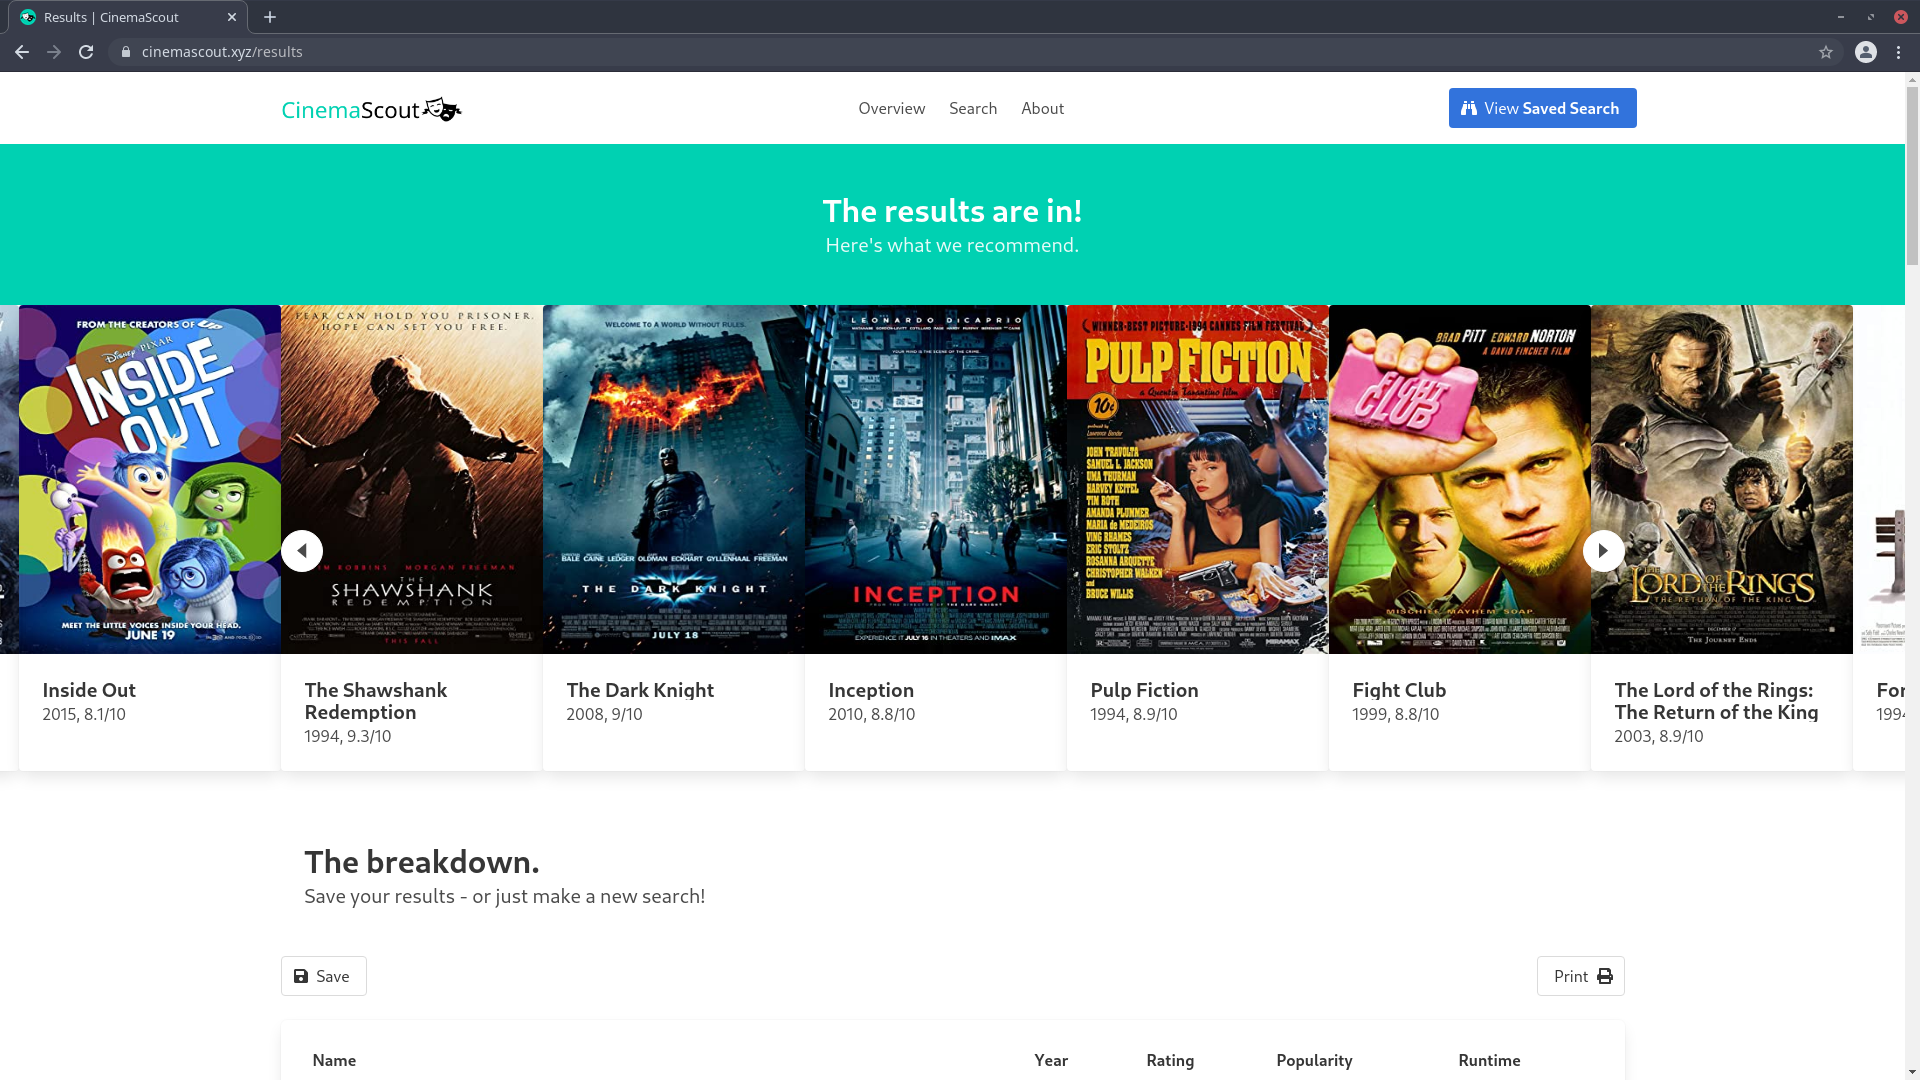
\includegraphics[width=\columnwidth]{res/results_0.png}
\caption{Results page, without further user input.}
\end{figure}
\begin{figure}[H]
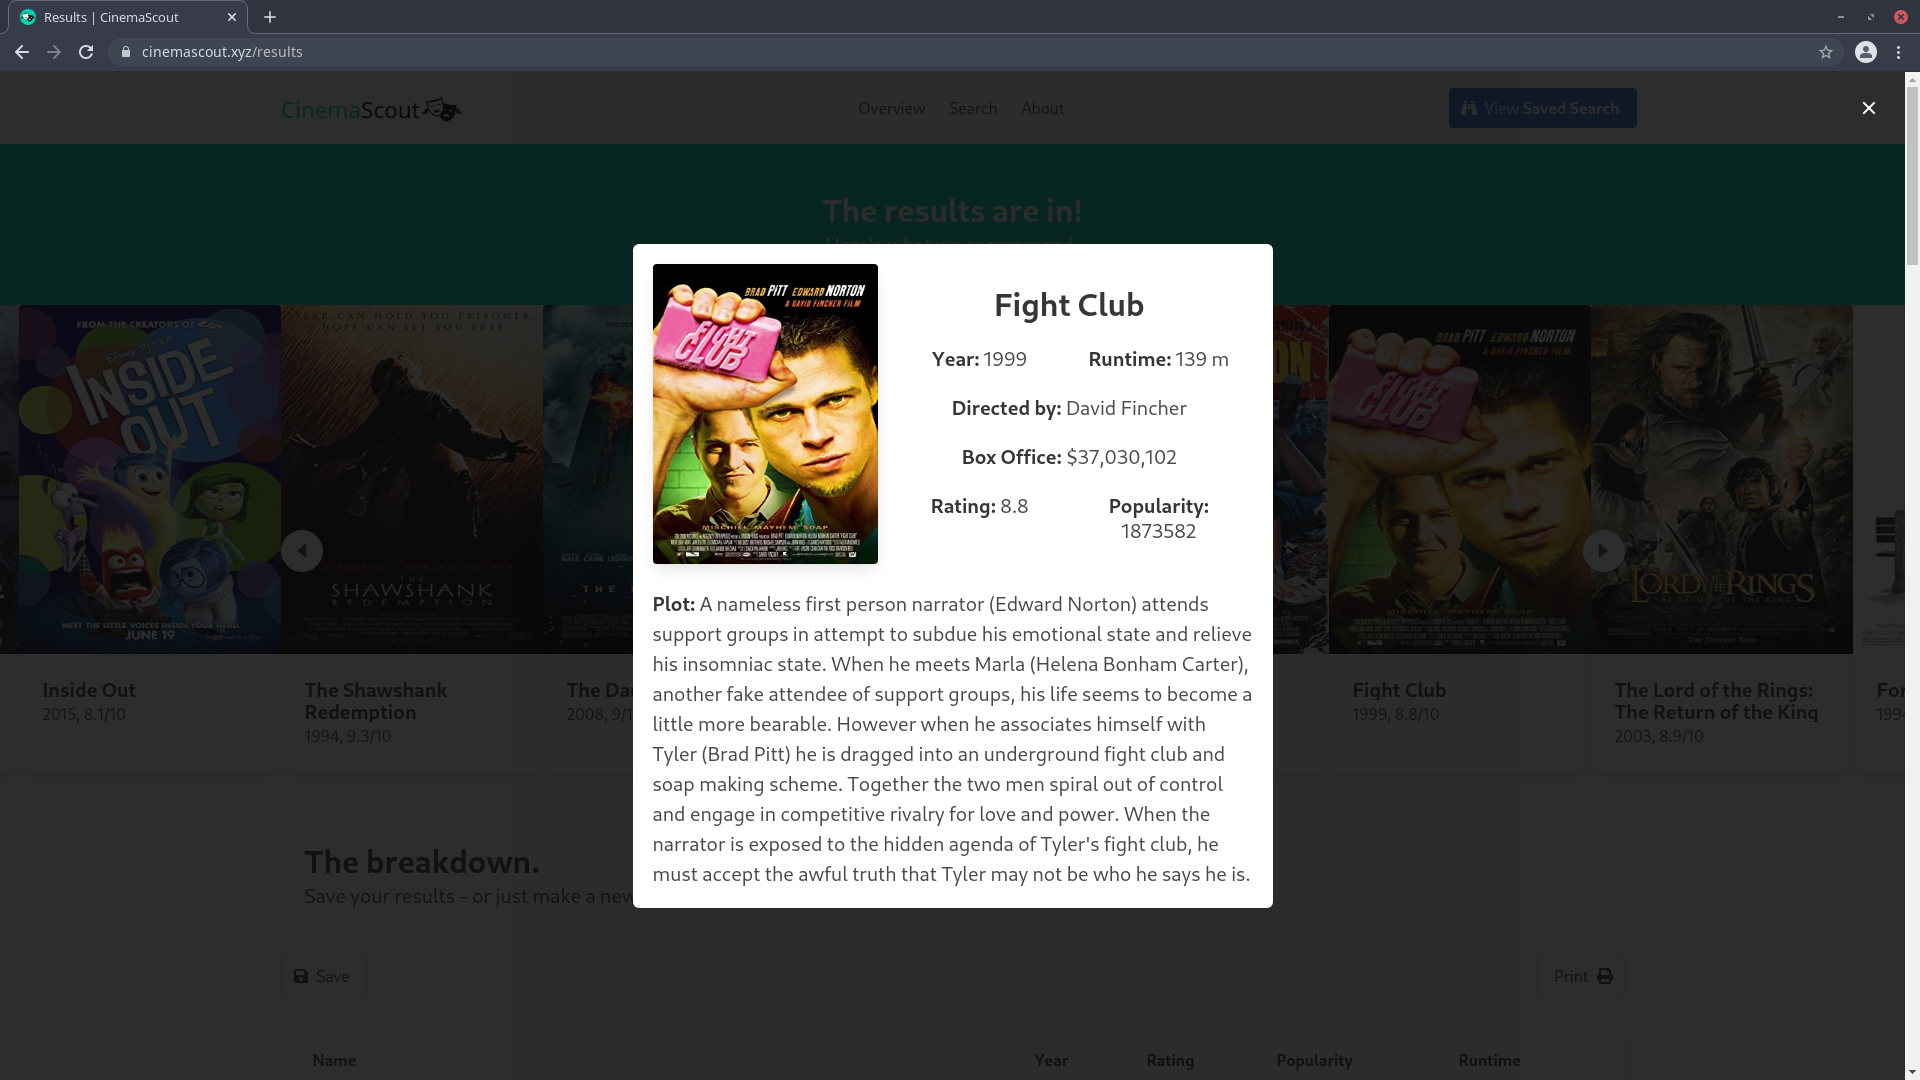
\includegraphics[width=\columnwidth]{res/results_1.png}
\caption{Results page after clicking on a movie and opening a modal.}
\end{figure}
\begin{figure}[H]
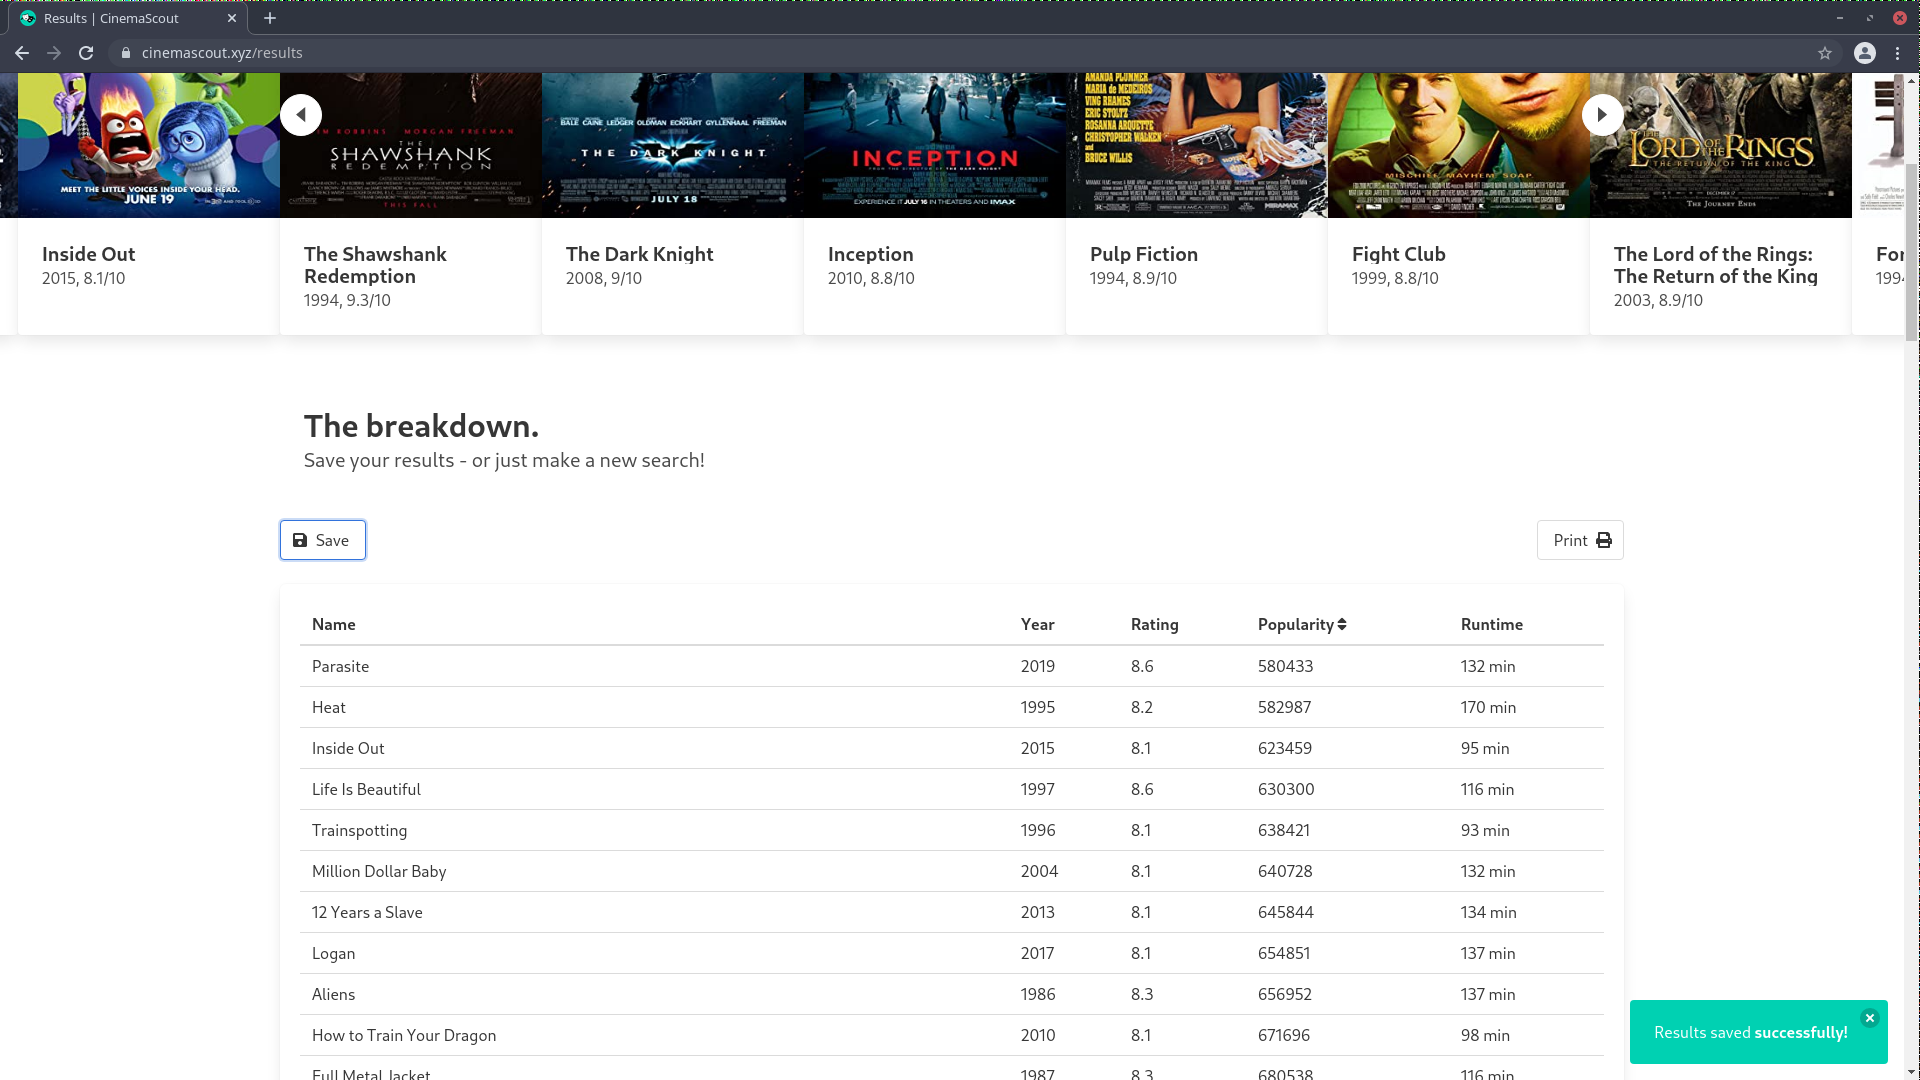
\includegraphics[width=\columnwidth]{res/results_2.png}
\caption{Results page after pressing save and sorting the table by runtime.}
\end{figure}
\begin{figure}[H]
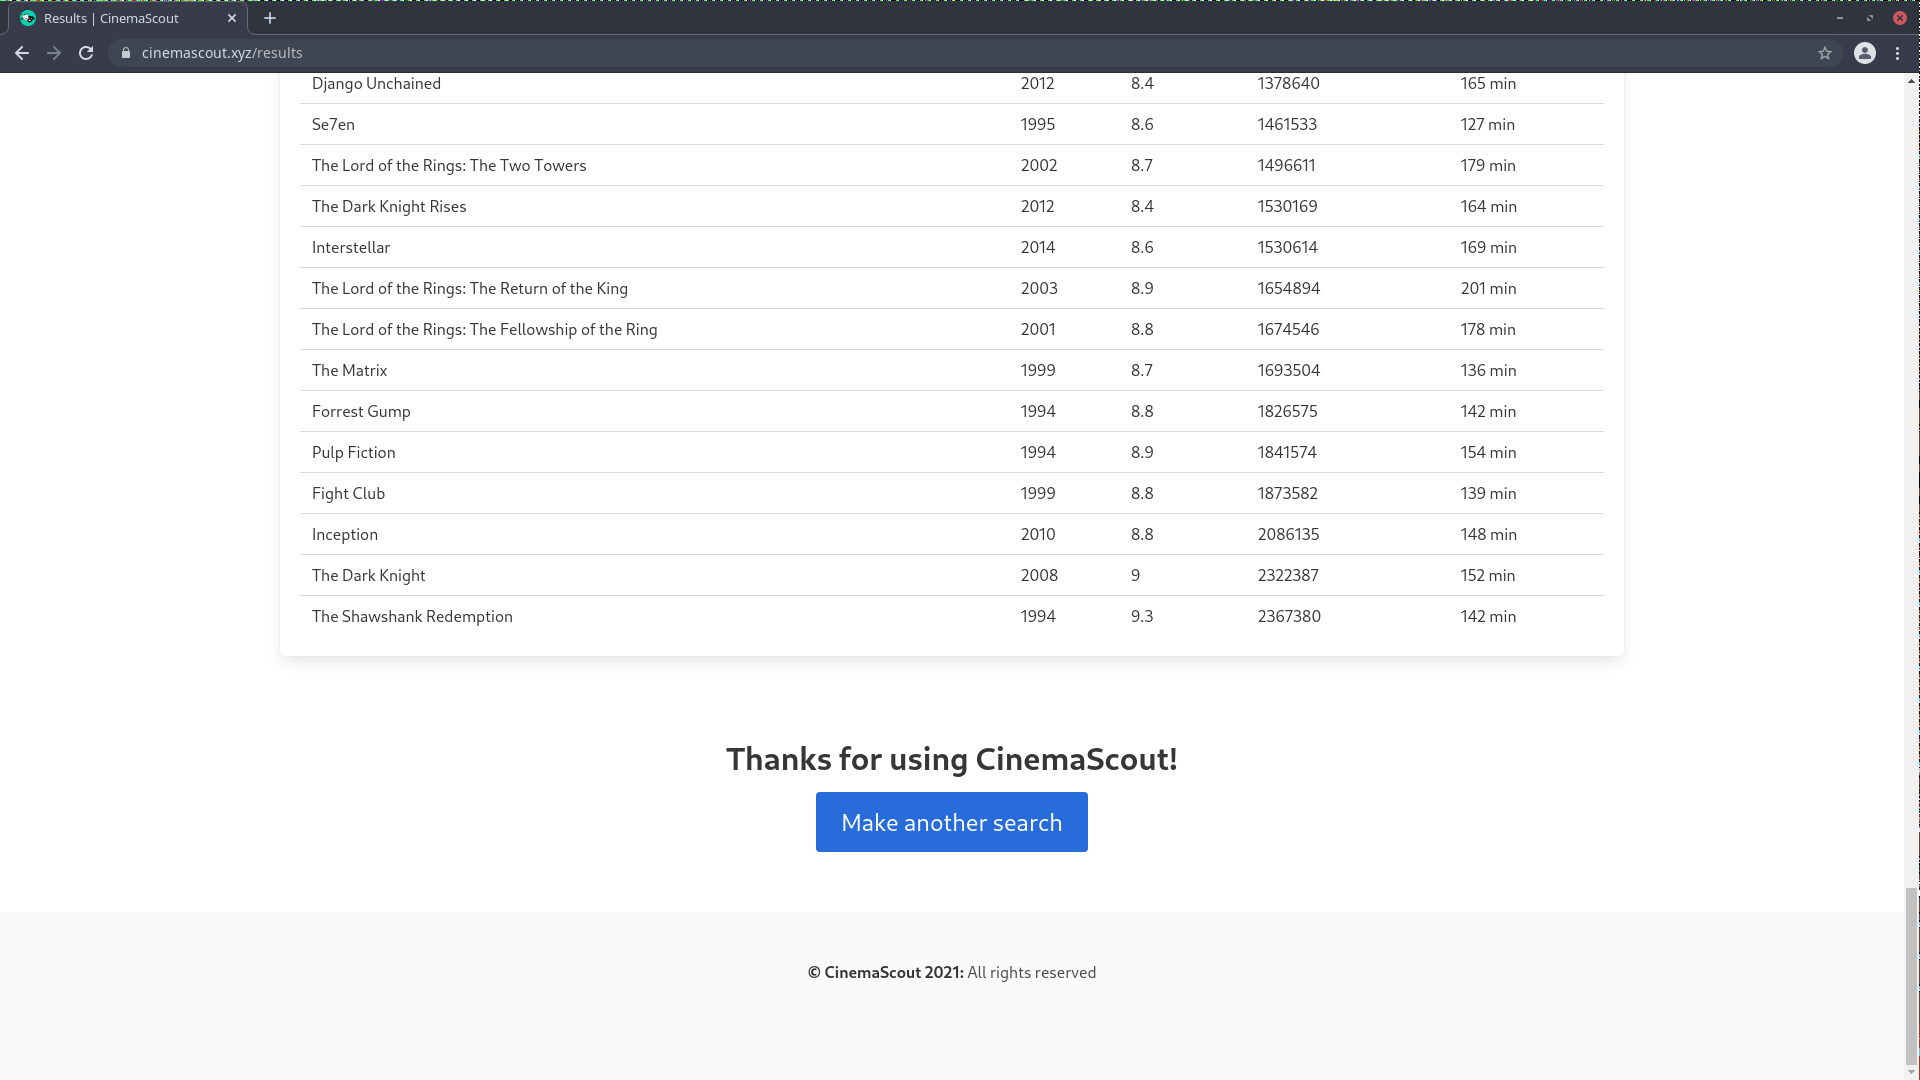
\includegraphics[width=\columnwidth]{res/results_3.png}
\caption{End of the results page.}
\end{figure}
\begin{figure}[H]
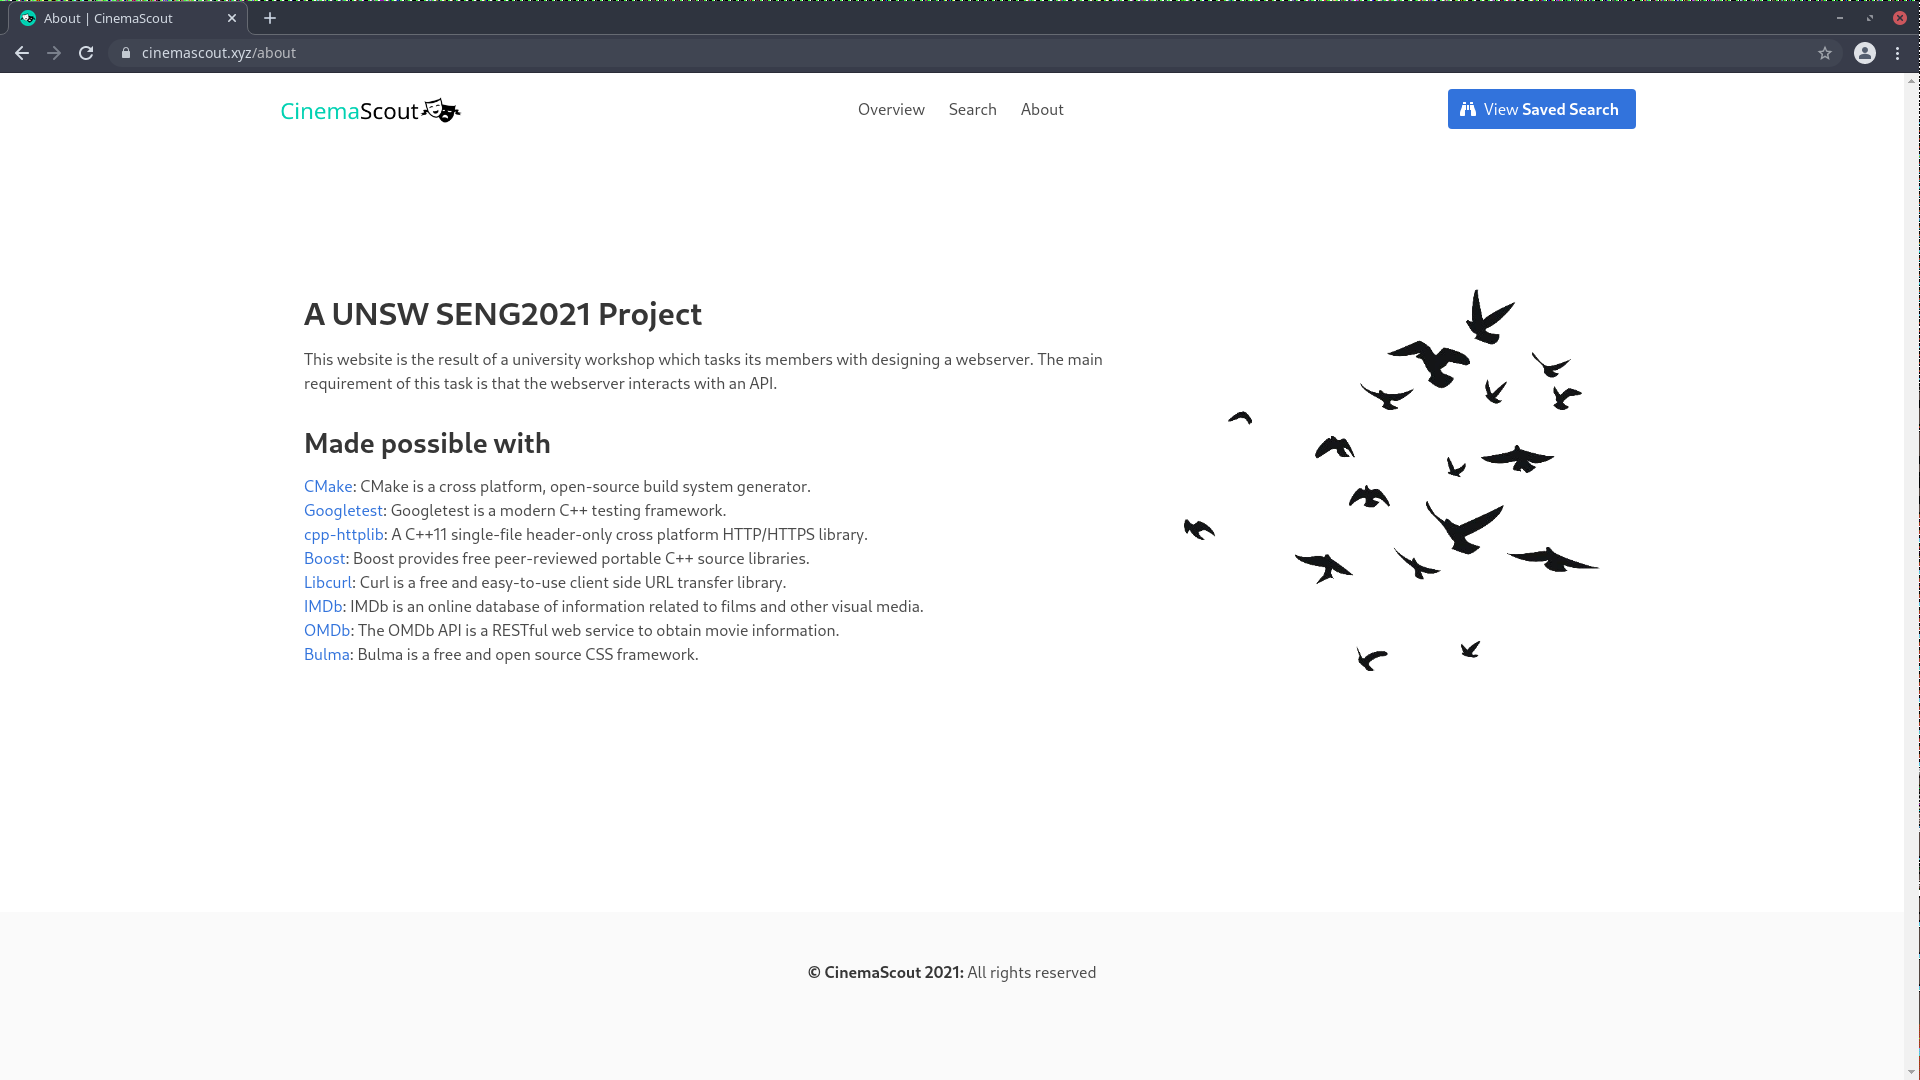
\includegraphics[width=\columnwidth]{res/about.png}
\caption{About page.}
\end{figure}
\newpage
\section{Part 2}
\subsection{Implementation Summary}
Foremost, the requirements for compiling, executing and maintaining the
CinemaScout webserver were actively reduced during software development in order
to minimise running costs and maximise profit potential. Consequently, the
choice of backend and frontend stack language targeted speed and efficiency over
ease of programming and simplicity. The backend stack was written in the 
statically typed C++ programming language while the frontend stack was written
in a combination of HTML5 (Hyper Text Markup Language 5), CSS (Cascading Style
Sheets) and JavaScript. In addition, a number of external dependencies were
introduced to reduce programming complexity, increase reliability and enable
a number of difficult operations for which it was not feasible to design given
the constrictive time limit in place. These include the following:
\subsubsection*{Build Dependencies}
\begin{itemize}
\item \textbf{CMake}: CMake is a cross platform, open-source build system
generator.
\item \textbf{Googletest}: Googletest is a modern C++ testing framework.
\item \textbf{cpp-httplib}: cpp-httplib is a C++11 single file cross platform
HTTP/HTTPS library.
\item \textbf{Boost}: Boost provides free peer-reviewed portable C++ source 
libraries.
\item \textbf{Libcurl}: Libcurl is a free and easy-to-use client side URL
transfer library.
\end{itemize}
\subsubsection*{Runtime Dependencies}
\begin{itemize}
\item \textbf{IMDb}: IMDb is an online database of information related to films
and other visual media.
\item \textbf{OMDb}: The OMDb API is a RESTful web service to obtain movie
information.
\item \textbf{Bulma}: Bulma is a free and open source CSS framework.
\end{itemize}
In general, operations made by the webserver backend may be split into either 
client or server modules. The client portion of the webserver, always loaded
directly after webserver execution, serves to populate the backend with data
so that the server portion may operate. The server module, interdependent with
the client portion, enables the serving of static files such as HTML5 or CSS
pages along with certain RESTful functionality such as GET and POST requests,
ultimately enabling the frontend to operate. Pertinently, an effort was made to
reduce network bandwidth to increase backend reliability, resulting in defensive
design choices such as the pre-caching of all potential API requests to OMDb so
that no API requests are made when the server is active.
\subsection{Software Architecture}
Placeholder.
\subsection{Sequence Diagrams}
The following sequence diagrams differ slightly from those of the previous
report to accomodate for design changes in the frontend user interface. 
Additionally, the sequence diagram for viewing movie trailers was removed 
entirely due to recent YouTube API restrictions making it infeasible to
implement.
\begin{figure}[H]
\includegraphics[width=\columnwidth]{res/sequence_diagram.png}
\caption{Typical CinemaScout Use Case.}
\end{figure}
\begin{figure}[H]
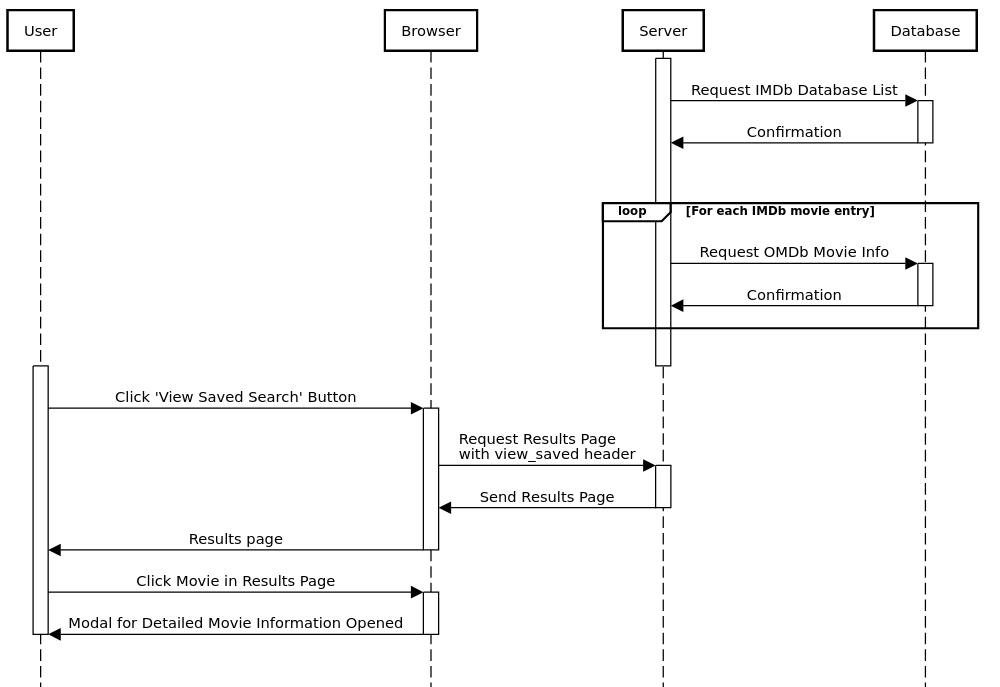
\includegraphics[width=\columnwidth]{res/sequence_diagram2.png}
\caption{View Saved Search Use Case.}
\end{figure}
\begin{figure}[H]
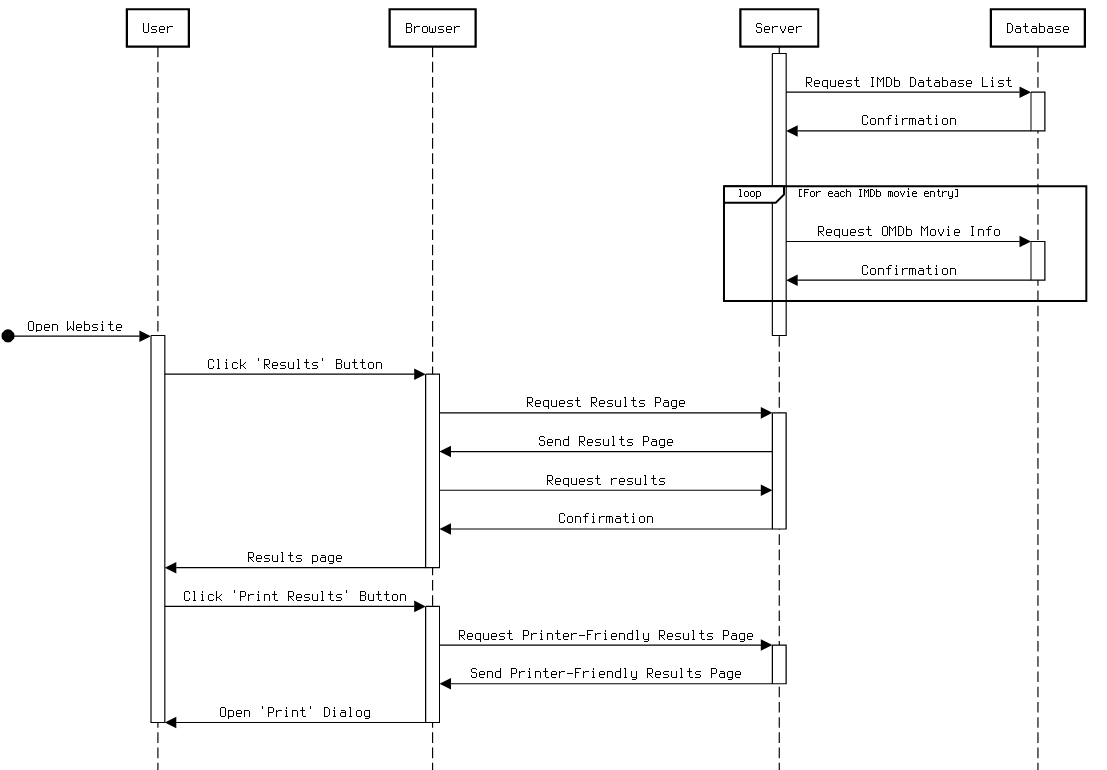
\includegraphics[width=\columnwidth]{res/sequence_diagram5.png}
\caption{Print Results Use Case.}
\end{figure}
\begin{figure}[H]
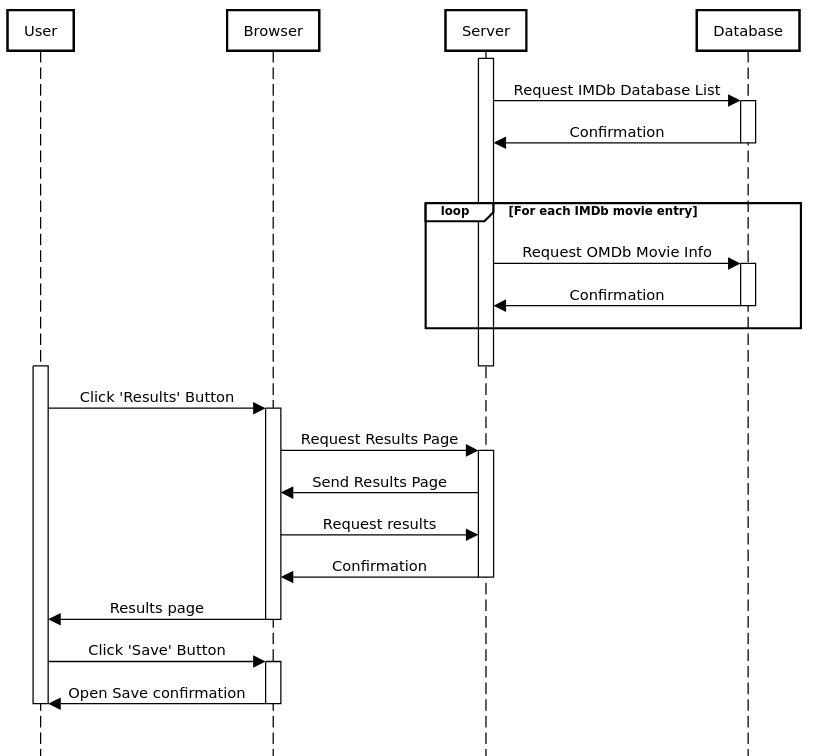
\includegraphics[width=\columnwidth]{res/sequence_diagram4.png}
\caption{Save Search Use Case.}
\end{figure}
\newpage
\subsection{Design Outcomes}
Placeholder.

\section{Part 3}
\subsection{Team Organisation}
Our team employed a flat organizational structure to meet the project's
requirements. Little to no hierarchy allowed the group to respond quicker
to emerging problems, as no formal permission was required by others for
a team member to begin working on an aspect of the project. The flat
organizational structure was particulary beneficial for the members of our
group due to differences in time zones between each group member, as
synchronous communication via direct meetings were problematic to organize.
As a result, any communication between group members was generally
asynchronous, typically occuring through the medium of text chat in Microsoft
Teams. In general, the responsibilities for each team member settled as:
\begin{itemize}
\item \textbf{Ben S}: Lead backend programmer; supporting frontend programmer
\item \textbf{Bowei P}: Algorithm specialist; frontend tester
\item \textbf{Nic S}: Lead frontend programmer; supporting backend programmer
\item \textbf{Ruqi L}: Deliverable maintaner; backend tester; quality
assurance
\end{itemize}
\subsection{Issues}
The project encountered both technical and non-technical issues. The backend,
initially powered with pistache for HTTP requests, was unsuitable for
deployment on any VPS due to the library's immaturity. Pistache is no longer
actively maintained, and suffers from several debilitating networking bugs
exposing the server to denial of service attacks. Additionally, the library is
not header-only, decreasing the server's portability among linux distributions
that do not supply packages for pistache. Switching to cpp-httplib, a
header-only and actively maintained HTTP library similar in design to python's
flask library rectified the issues. Similarly, the dated design of rapidjson, a
library for managing JSON objects used in the backend to categorise movie data,
reduced the readability of the codebase. Alternatives with greater readability
suffered from weak performance, and were deemed unsuitable. The interface of
rapidjson was convoluted to the point that some of the server code manipulated
JSON objects with raw strings rather than via rapidjson's API, resulting in
a degree of code duplication. The documentation of rapidjson is largely
incomplete, and several server bugs were the result of incorrect assumptions
regarding the thread safety of several rapidjson operations.\\
The main non technical issues encountered by the group were due to real world
circumstances. During the final stages of the project, half of the team were
without a stable internet connection due to a change in living arrangements.
Careful planning was required to synchronise project due dates with periods
of time when utilities were available. Most prominently, the move of house
was planned to occur a day after deliverable 4 - the online, live demonstration
of the project. Additionally, the distributed location of several group members
across several time zones complicated team communcation. To rectify the issue,
asynchronous communication was relied upon for the entirety of the project.
 
\subsection{Project Reflection}
The team is satisfied with the result of the project, and substantial
experience has been gained by reflecting on issues encountered during the
project's development.\\
The team has learned to carefully analyse and vet all project dependencies
before including them in the codebase, as they can quickly become a permanent
fixture in the software's design. Had the dependency not meet expectations,
the project can become significantly impeded, as development time required
to find and integrate a replacement prevents the project from maturing in
other directions. Dependencies should all be checked to have acceptable
licensing, performance and reliability, preferably via real-world tests, before
they are to be considered for inclusion in the project.\\
The ability to adapt to change is particularly relevant within the field of
software engineering. The decentralised and online nature of programming can
result in unconventional team situations and work environments.
It is an essential skill for engineers to be proficient in communicating
effectively both in person and via online mediums, through both synchronous and
asynchronous methods. Failing to adapt to changes in work situations can result
in a lack of team cohesion and the failure of a project.

\end{document}
